\section{Details of Multitenancy Stress Tests}
\label{appendix:multitenancy}

In multitenancy tests we are interested in examining the behavior of the systems under heavy and dynamic query load.
This simulates a common deployment in which the Accumulo cluster is a shared resource backing a group of application servers.
The benchmark service acts as our application server, receiving the full query result-set and producing a digested view for the client.
We've formulated this test to make the Accumulo cluster and its SimpleFeature index the only contested resource.

\subsection{Setup}

The client query load is provided by Gatling load-testing tool (\url{http://gatling.io}) issuing HTTP requests against a load-balanced group of application servers.
In turn these application servers query the Accumulo cluster to produce a  summary result for the client and log the query execution time.
Gatling allows us to maintain a constant number of concurrent query connections.
A connection is considered active until the benchmark services iterates over the query results set or a time-out of $60$ seconds.

As with other tests the benchmark service saves the query timings, which happens even in the event of a time-out on the client/benchmark-server connection.
However, unlike the earlier test-ups all the queries per scenario are done against either GeoMesa or GeoWave -- not both.
This produces a reliable and uninterrupted load on the target system.

\subsection{GDELT}

The queries are executed against GDELT ingested into a cluster with $5$ workers as in previous tests.
We reuse the City Buffers queries, as well as the queries against South American countries,
randomly selecting parameters for spatial and temporal bounds.
Up to eight concurrent connections for each query group will be open with no pause between subsequent requests.
This is a very dynamic load test as the City Buffers queries span up fourteen months and the South America queries will issue twelve DataStore queries for every HTTP request.

Our initial tests have produced a surprising differentiation between the two systems.
In this scenario GeoWave was able to process a $3.5 \times$ higher request volume than GeoMesa.
Also during this time we witnessed two instances where GeoMesa clusters entered degraded performance mode,
where query duration seems to increase permanently after a round of load testing.
After increasing the accumulo memory allocations as described below the performance gap shrunk, with GeoWave delivering $30$\% higher request volume.

\subsubsection{Test Results}

Because the Accumulo-backed DataStore can receive records from multiple tablet servers the application server network interface can easily become saturated.
As a start we re-ran the tests with increasing the number of application servers to remove this bottleneck and increase the query throughput until the cluster under test becomes the limiting resource.
Because small client queries trigger large query workloads we do not consider the connection between application server and Gatling client a limited resource.

We are interested in how concurrency impacts the duration of query execution.
The number of concurrent queries at the time of submission is calculated based on query start and end times as recorded by the application service.
Before each round of testing we verified that all clusters were idle, not undergoing any compactions or scans.

{\bf Configuration 1: 1 Application Server.}
This configuration is expected to degenerate; a single application server does not have the network bandwidth to pull the requested records and we see query duration spike well past usual levels.
From the client perspective this scenario produced cumulative timeout rates of about $50$\% for both systems.
After this round of testing GeoMesa cluster experienced an unexpected severity of degradation in query performance.
This prompted us to bring up two replacements for future tests.
Please see Figure \ref{config1}.

\begin{figure}[h!tb]
  \centering
  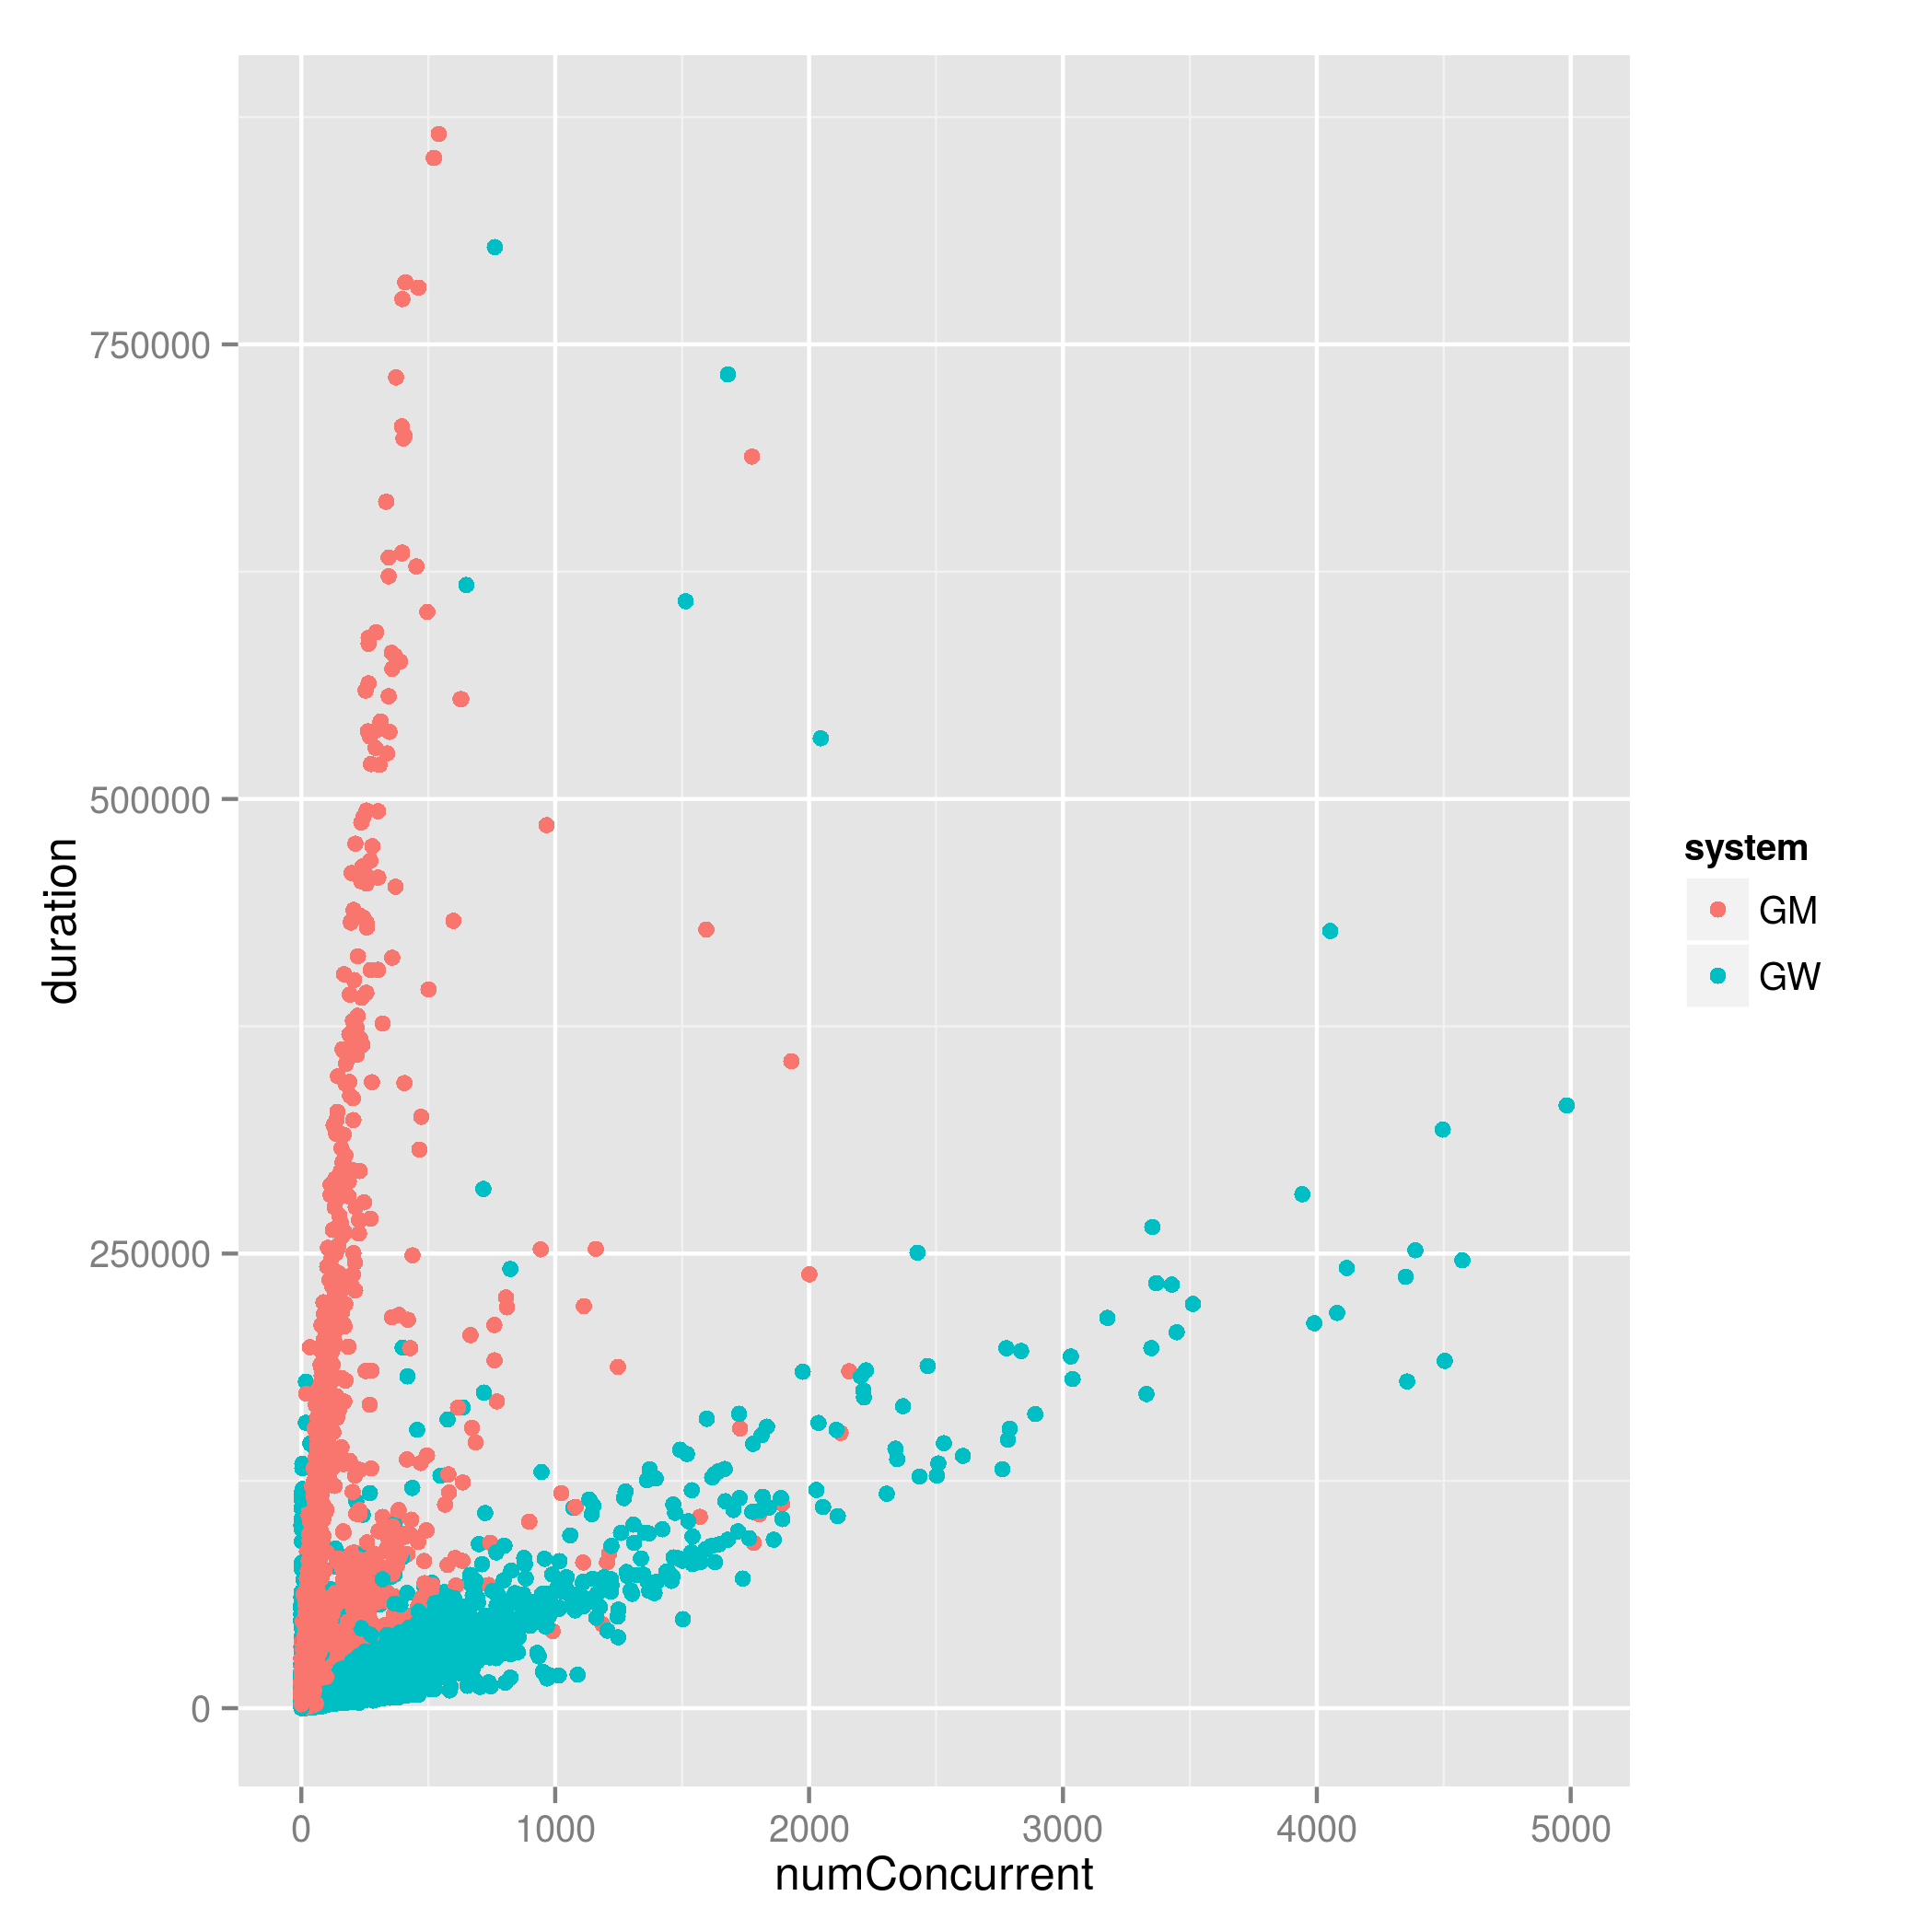
\includegraphics[width=0.60\textwidth]{../docs/img/multitenancy/graph_uncut_mt1.png}
  \caption{GDELT multitenancy results, configuration 1.}
  \label{config1}
\end{figure}

{\bf Configuration 2: 4 Application Servers.}
With four application servers we expect the network to no longer constrain the query execution.
Notably we see that GeoMesa is working against higher concurrency and producing higher delays.
These effects are likely mutually-reinforcing.
From the client we saw the query timeouts drop to $ \approx 5$\% for GeoWave and remain at $\approx 20$\% for GeoMesa.
These results contain two GeoMesa clusters and we do not see the effects of performance degradation from the \texttt{MT1} test.
Please see Figure \ref{config2}.

\begin{figure}[h!tb]
  \centering
  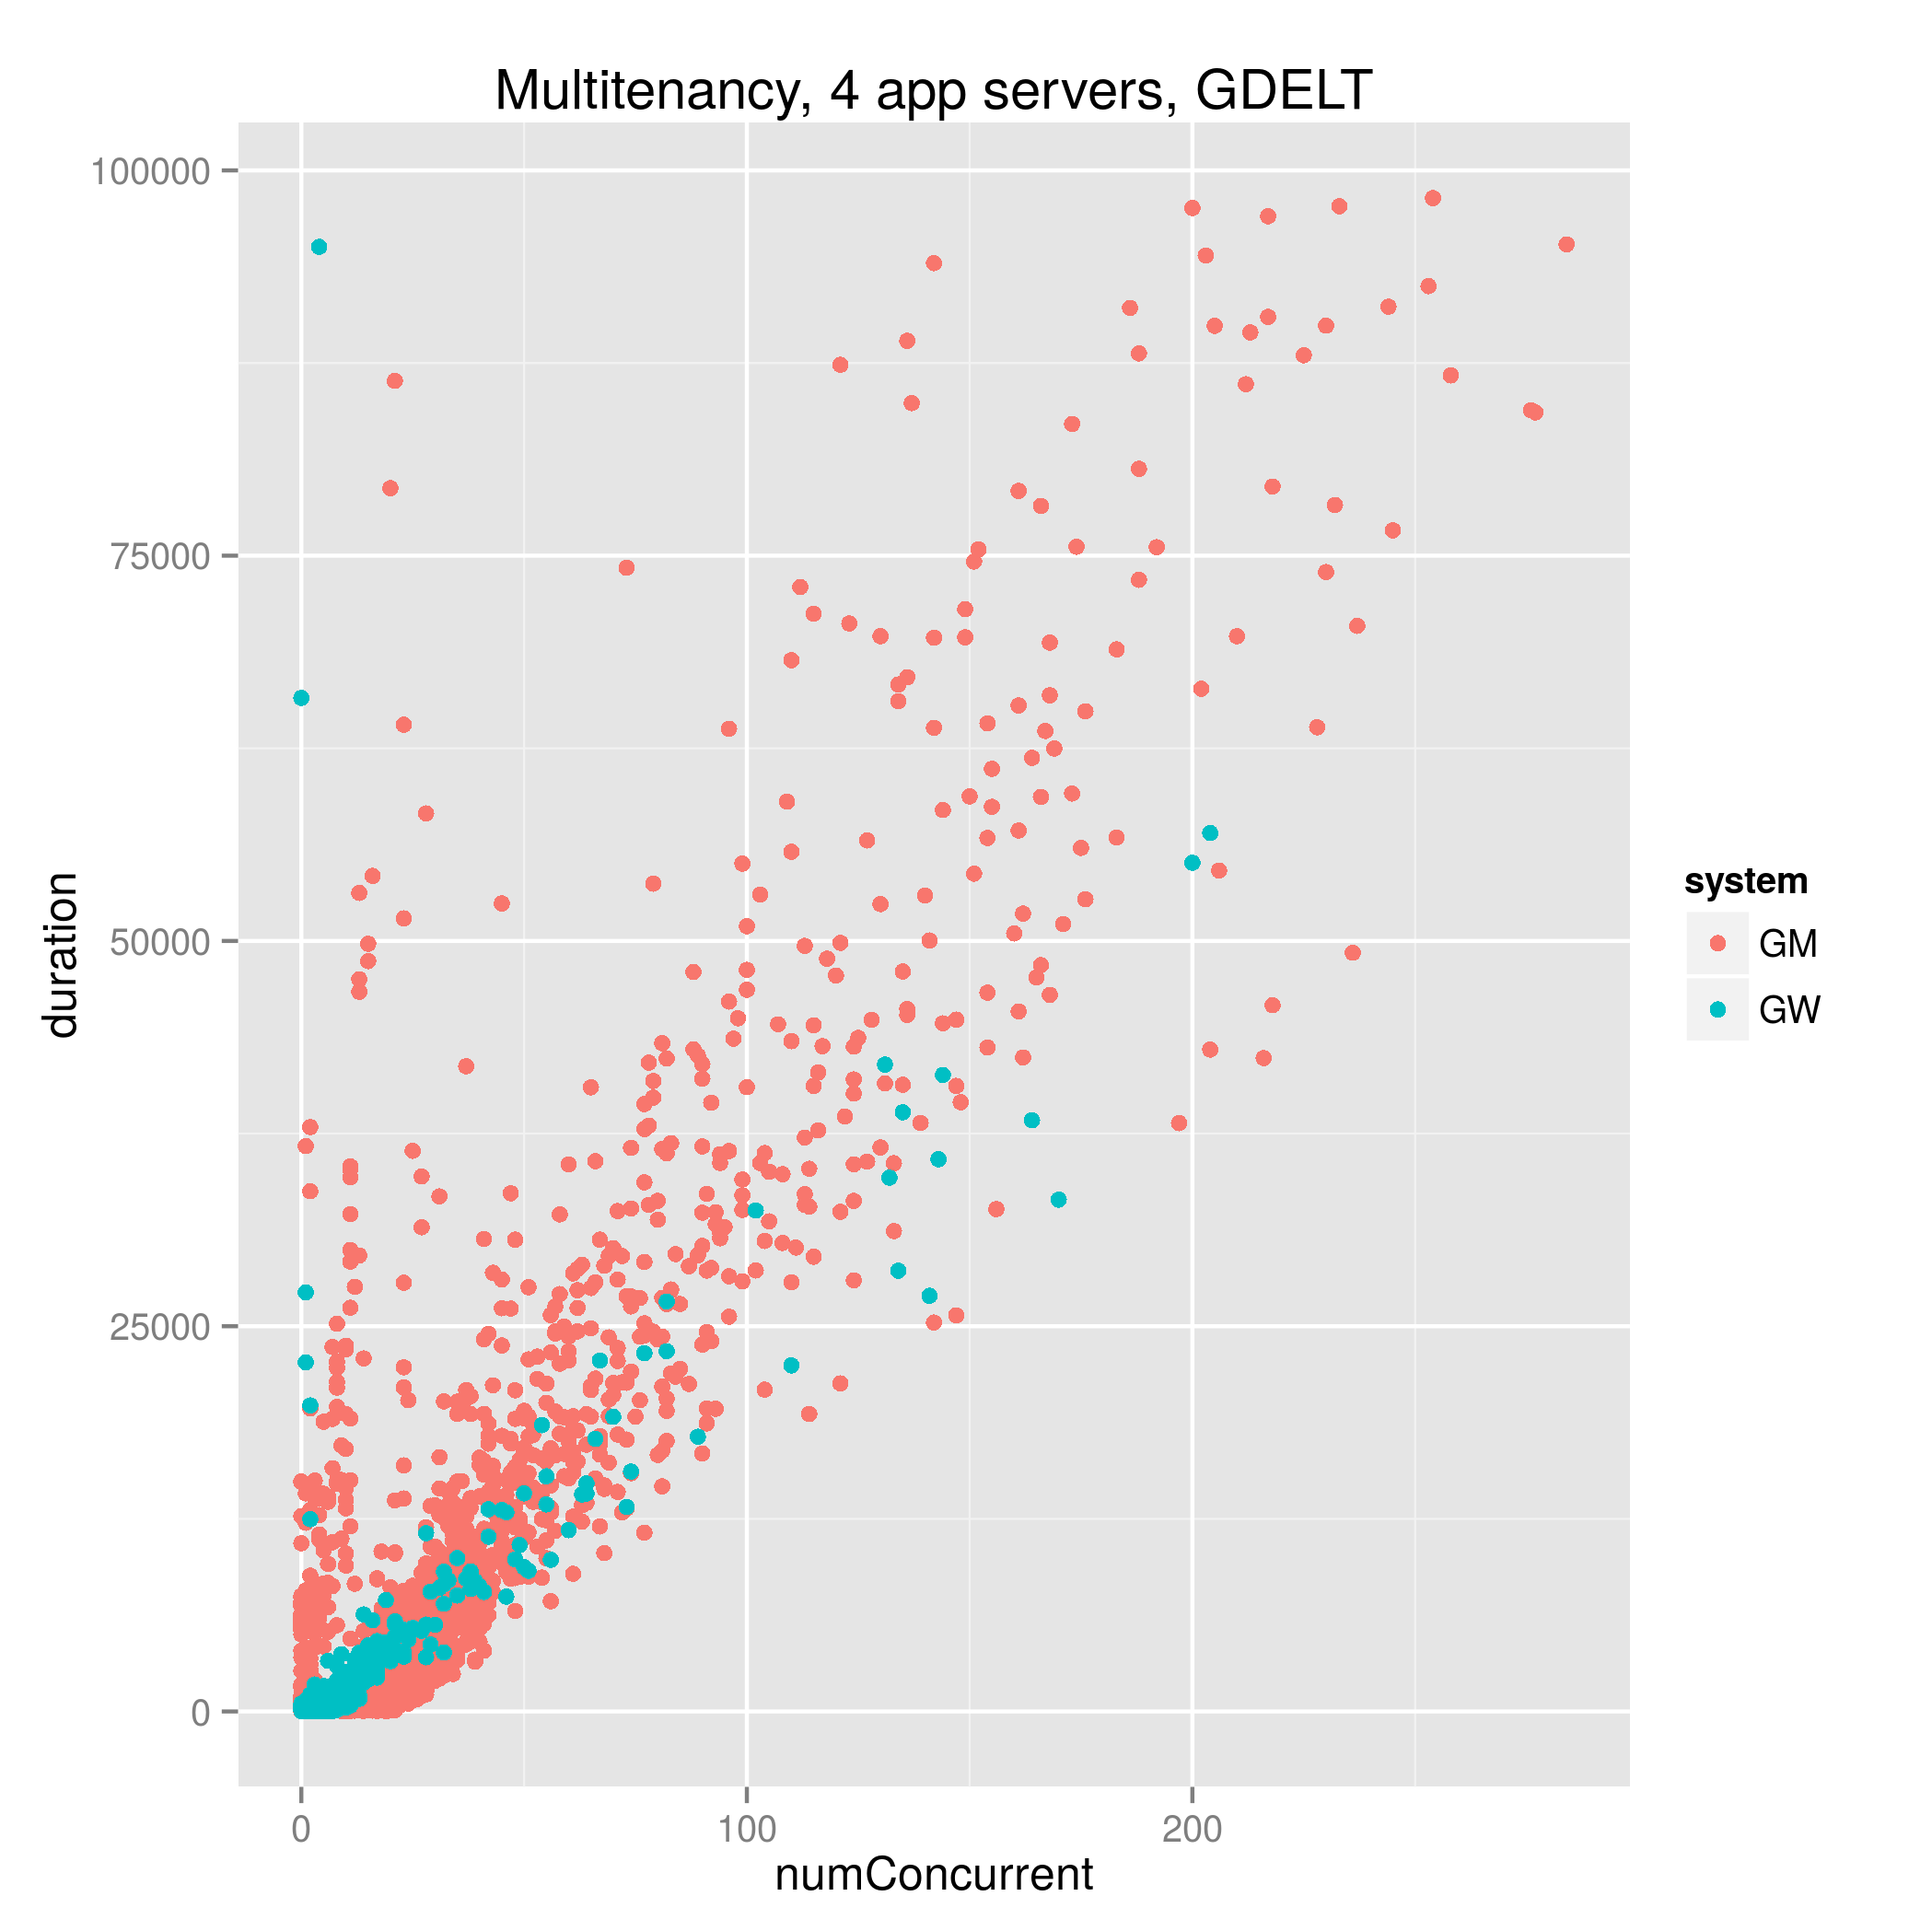
\includegraphics[width=0.60\textwidth]{../docs/img/multitenancy/graph_100k_mt2.png}
  \caption{GDELT multitenancy results, configuration 2.}
  \label{config2}
\end{figure}

{\bf Configuration 3: 6 Application Servers.}
We increase the application server count to six to verify that we have removed any performance impact from this parameter,
as we expect the duration and concurrency distributions remain consistent, indicating that in both \texttt{MT2} and \texttt{MT3} results the cluster resources are the only remaining constraint.
However, at this point one of the two GeoMesa clusters started experiencing similar performance degradation as after \texttt{MT1} round of tests.
This can be seen as two distinct distributions of GeoMesa results.
Please see Figures \ref{config3}, \ref{config3distrogw}, and \ref{config3distrogm}.

\begin{figure}[h!tb]
  \centering
  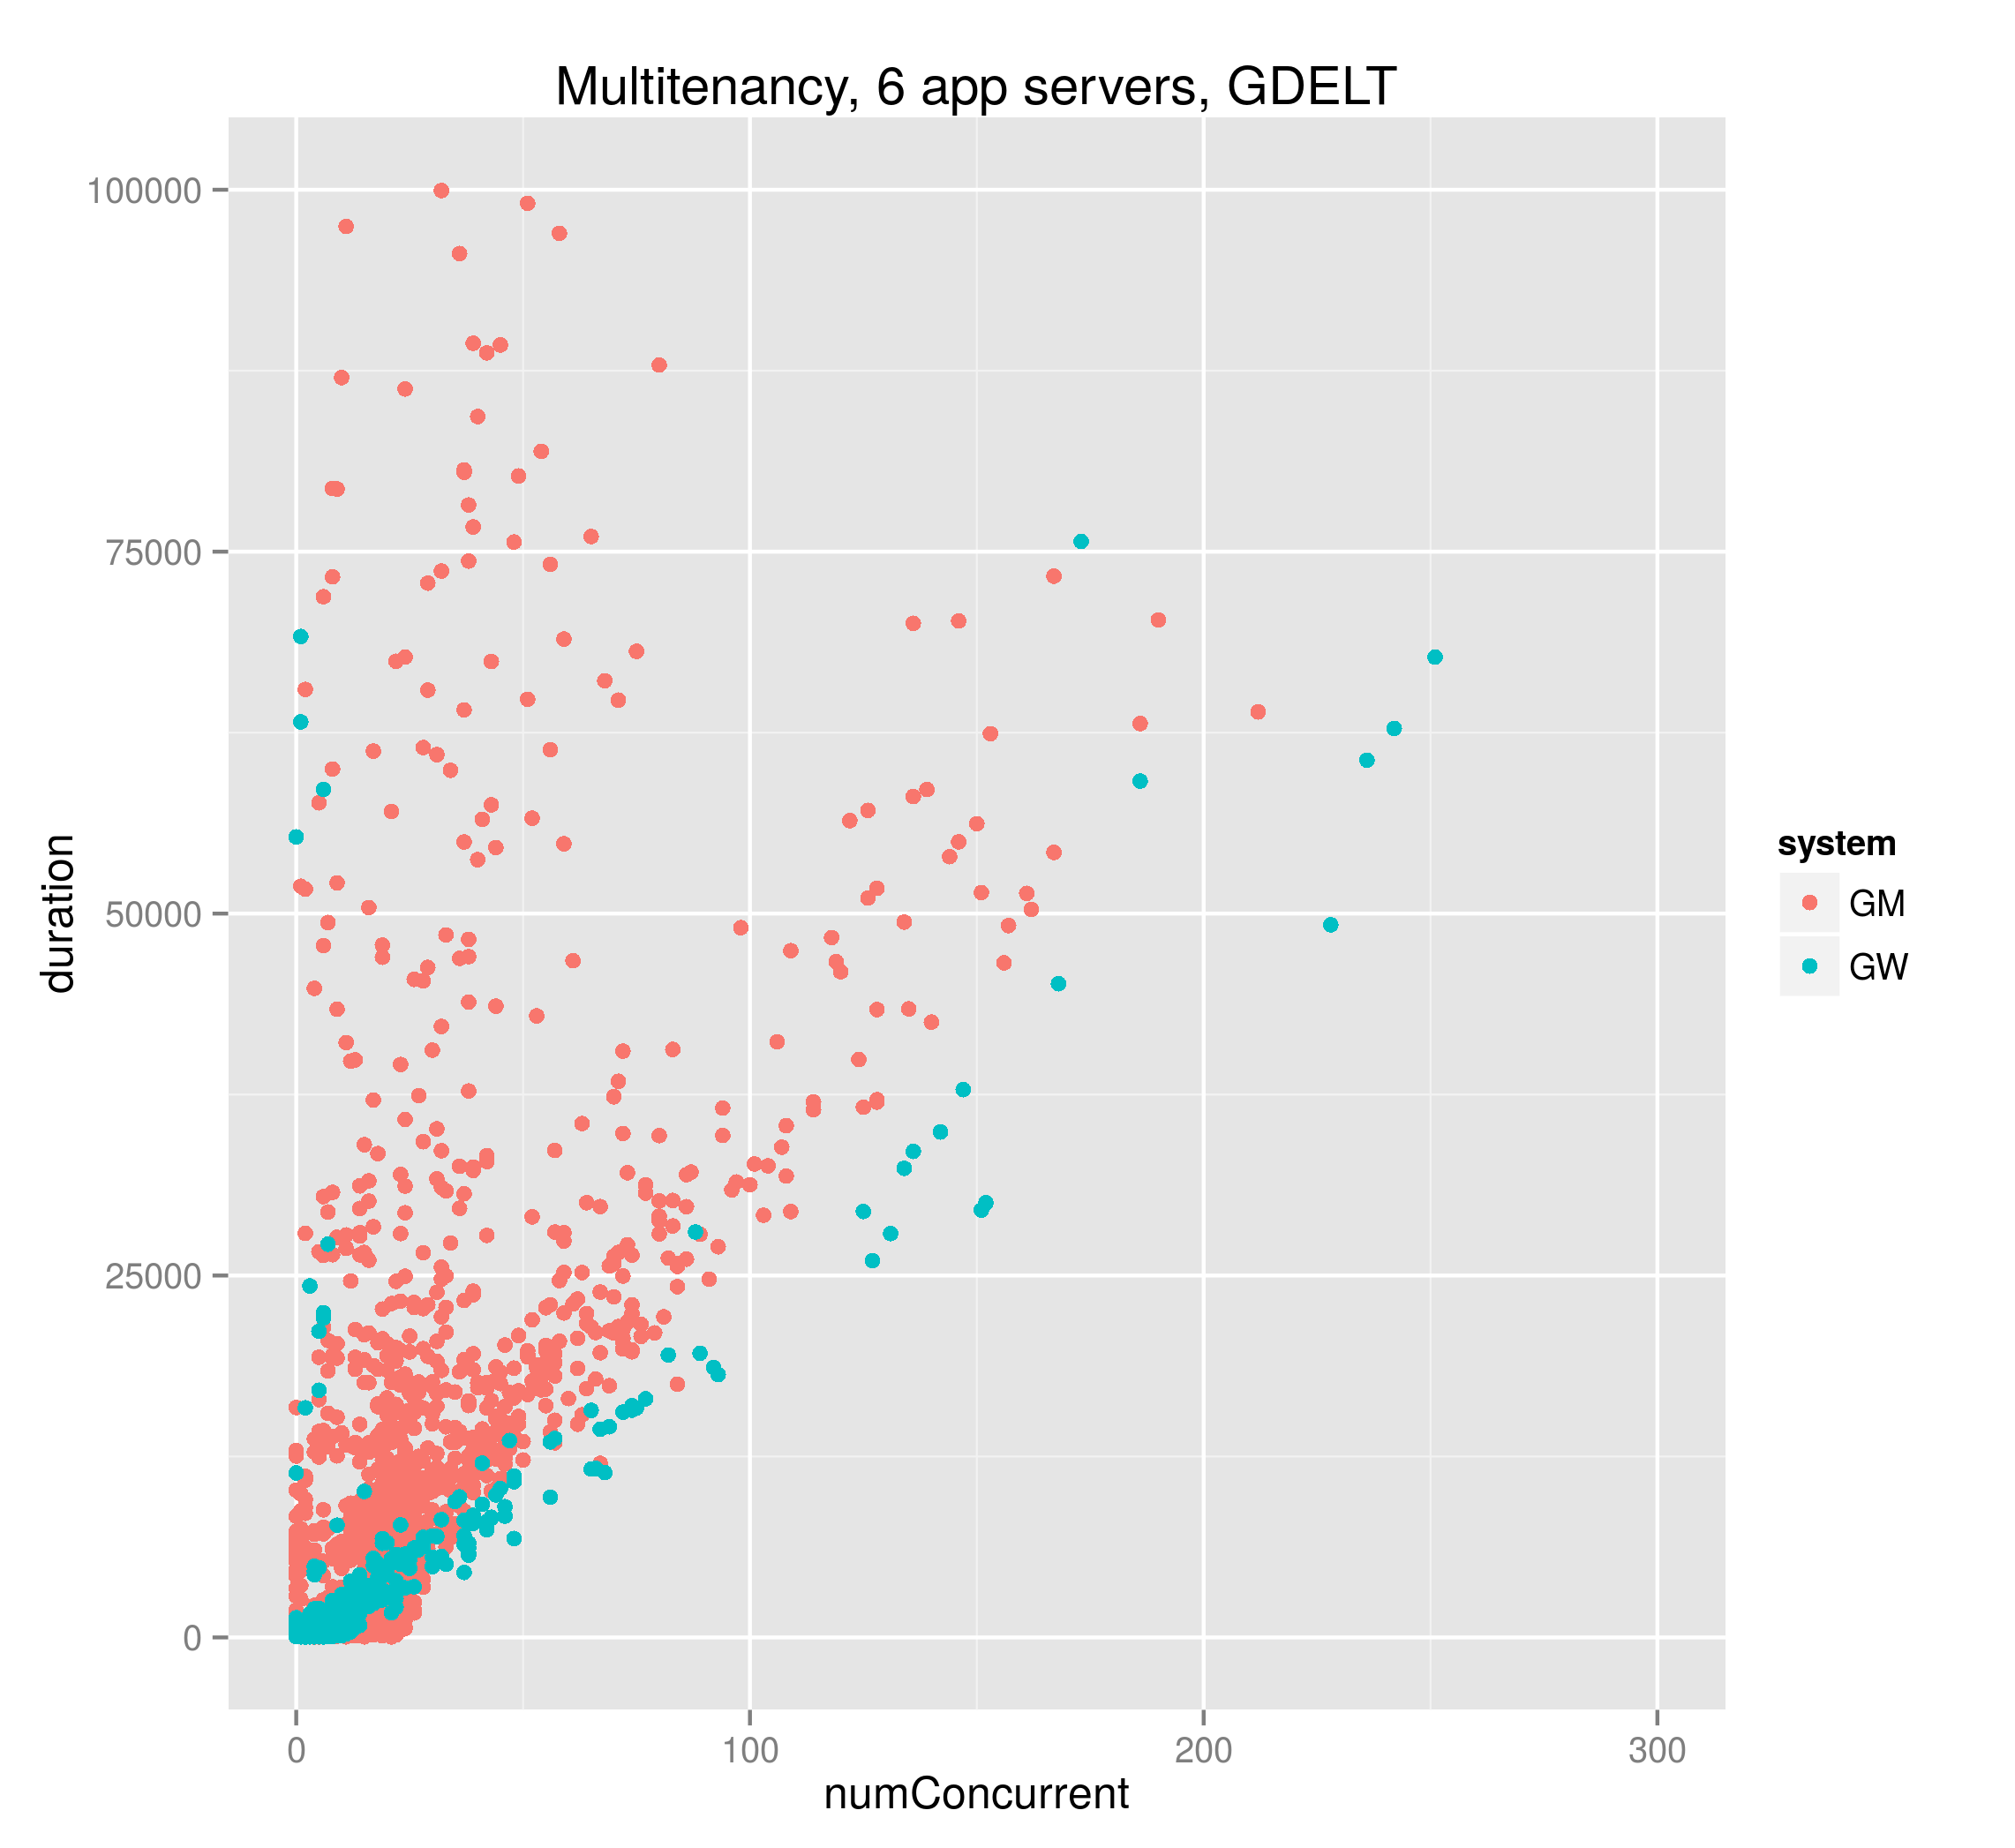
\includegraphics[width=0.60\textwidth]{../docs/img/multitenancy/graph_100k_mt3.png}
  \caption{GDELT multitenancy results, configuration 3.}
  \label{config3}
\end{figure}

\begin{figure}[h!tb]
  \centering
  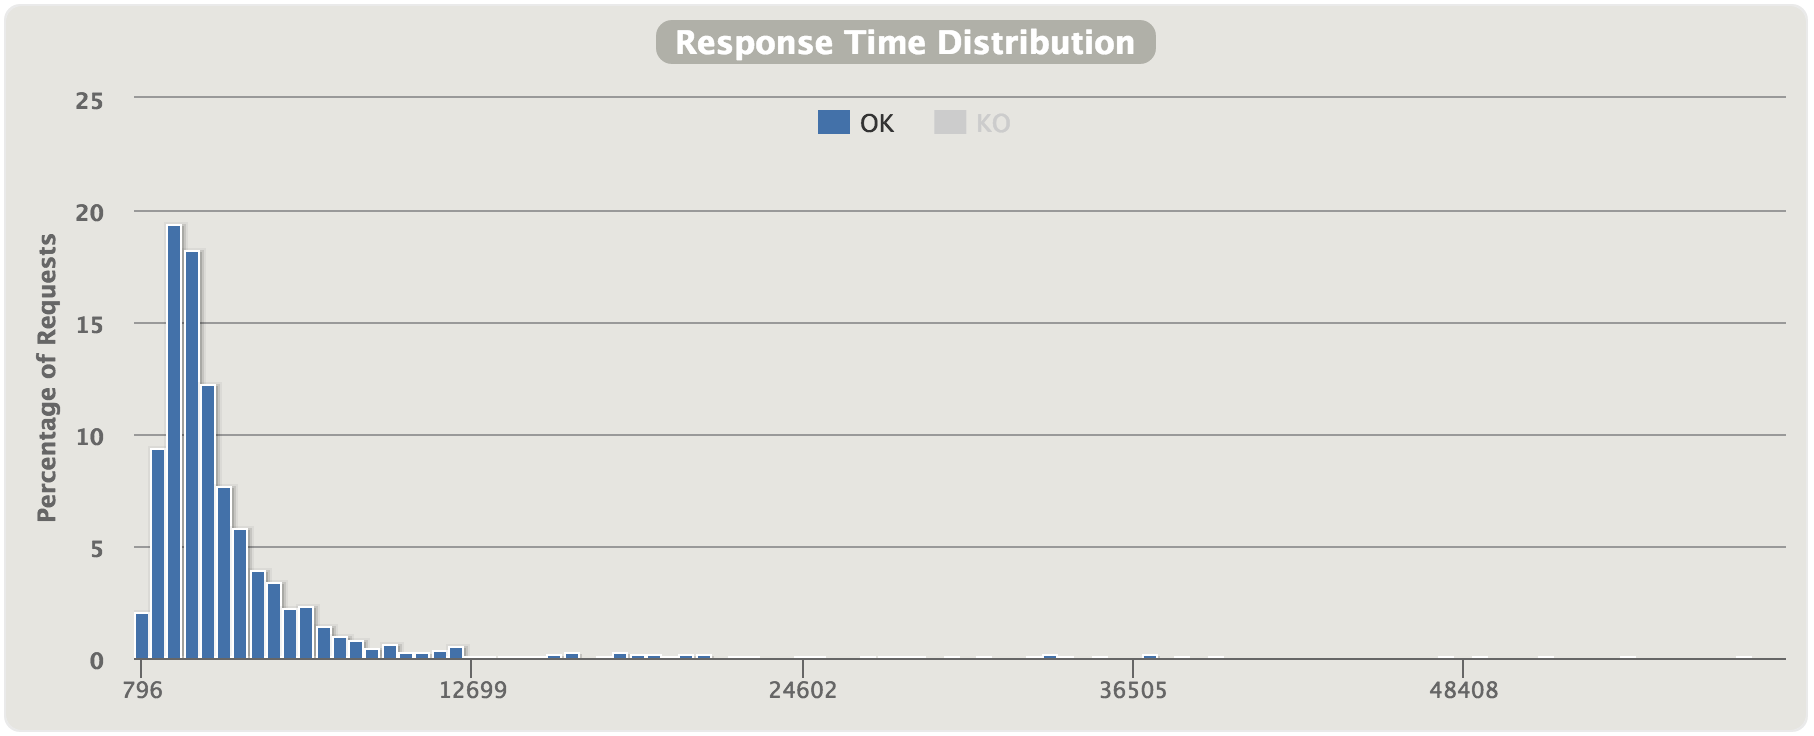
\includegraphics[width=0.60\textwidth]{images/mt3-2-gw.png}
  \caption{GeoWave/GDELT response times, configuration 3.}
  \label{config3distrogw}
\end{figure}

\begin{figure}[h!tb]
  \centering
  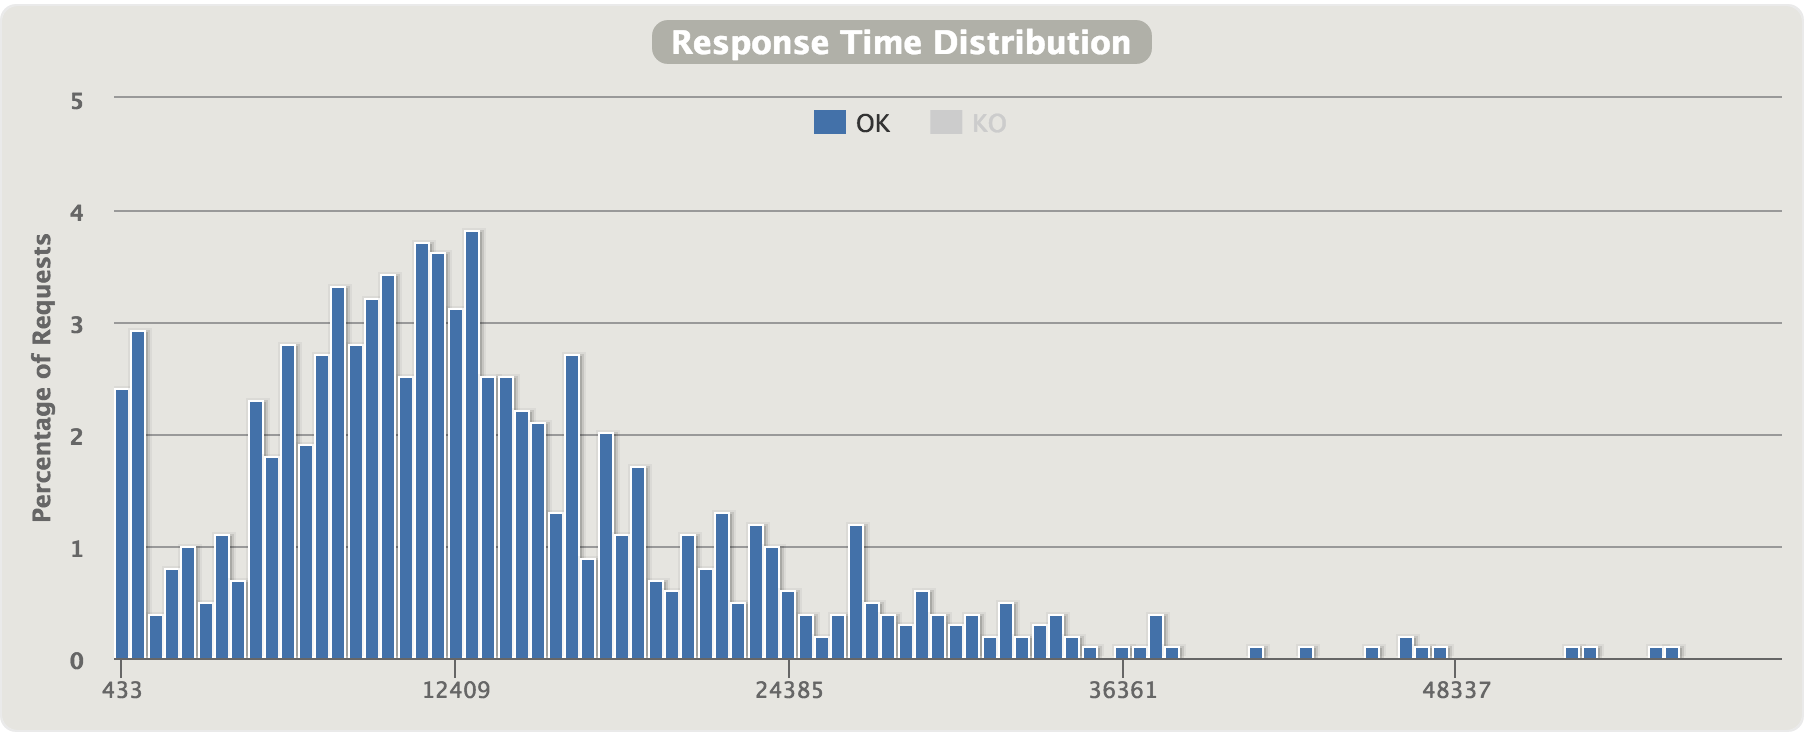
\includegraphics[width=0.60\textwidth]{images/mt3-2-gm.png}
  \caption{GeoMesa/GDELT response times, configuration 3.}
  \label{config3distrogm}
\end{figure}

\subsubsection{Troubleshooting GeoMesa Performance}

Based on input from GeoMesa team we increased the Accumulo memory configurations,
as shown in Table \ref{table:troubleshoot},
and re-ran the benchmark with six application servers for both systems.

\begin{table}[h!tb]
  \centering
  \begin{tabular}{ | l | c c | }
    \hline
    & Initial & Updated \\
    \hline
    \multicolumn{3}{| l |}{CONFIGURATION} \\ \hline
    master JVM -Xmx & $2$G & $3$G \\ \hline
    tserver JVM -Xmx & $3$G & $24$G \\ \hline
    tserver.cache.data.size & $128$M & $16$G \\ \hline
    tserver.cache.index.size & $128$M & $4$G \\ \hline
    \multicolumn{3}{| l |}{RESULTS} \\ \hline
    GeoWave Query Volume & $3072$ & $2808$ \\ \hline
    GeoMesa Query Volume & $863$ & $2107$ \\ \hline
  \end{tabular}
  \caption{GDELT multitenancy Accumulo memory configurations.}
  \label{table:troubleshoot}
\end{table}

\begin{figure}[h!tb]
  \centering
  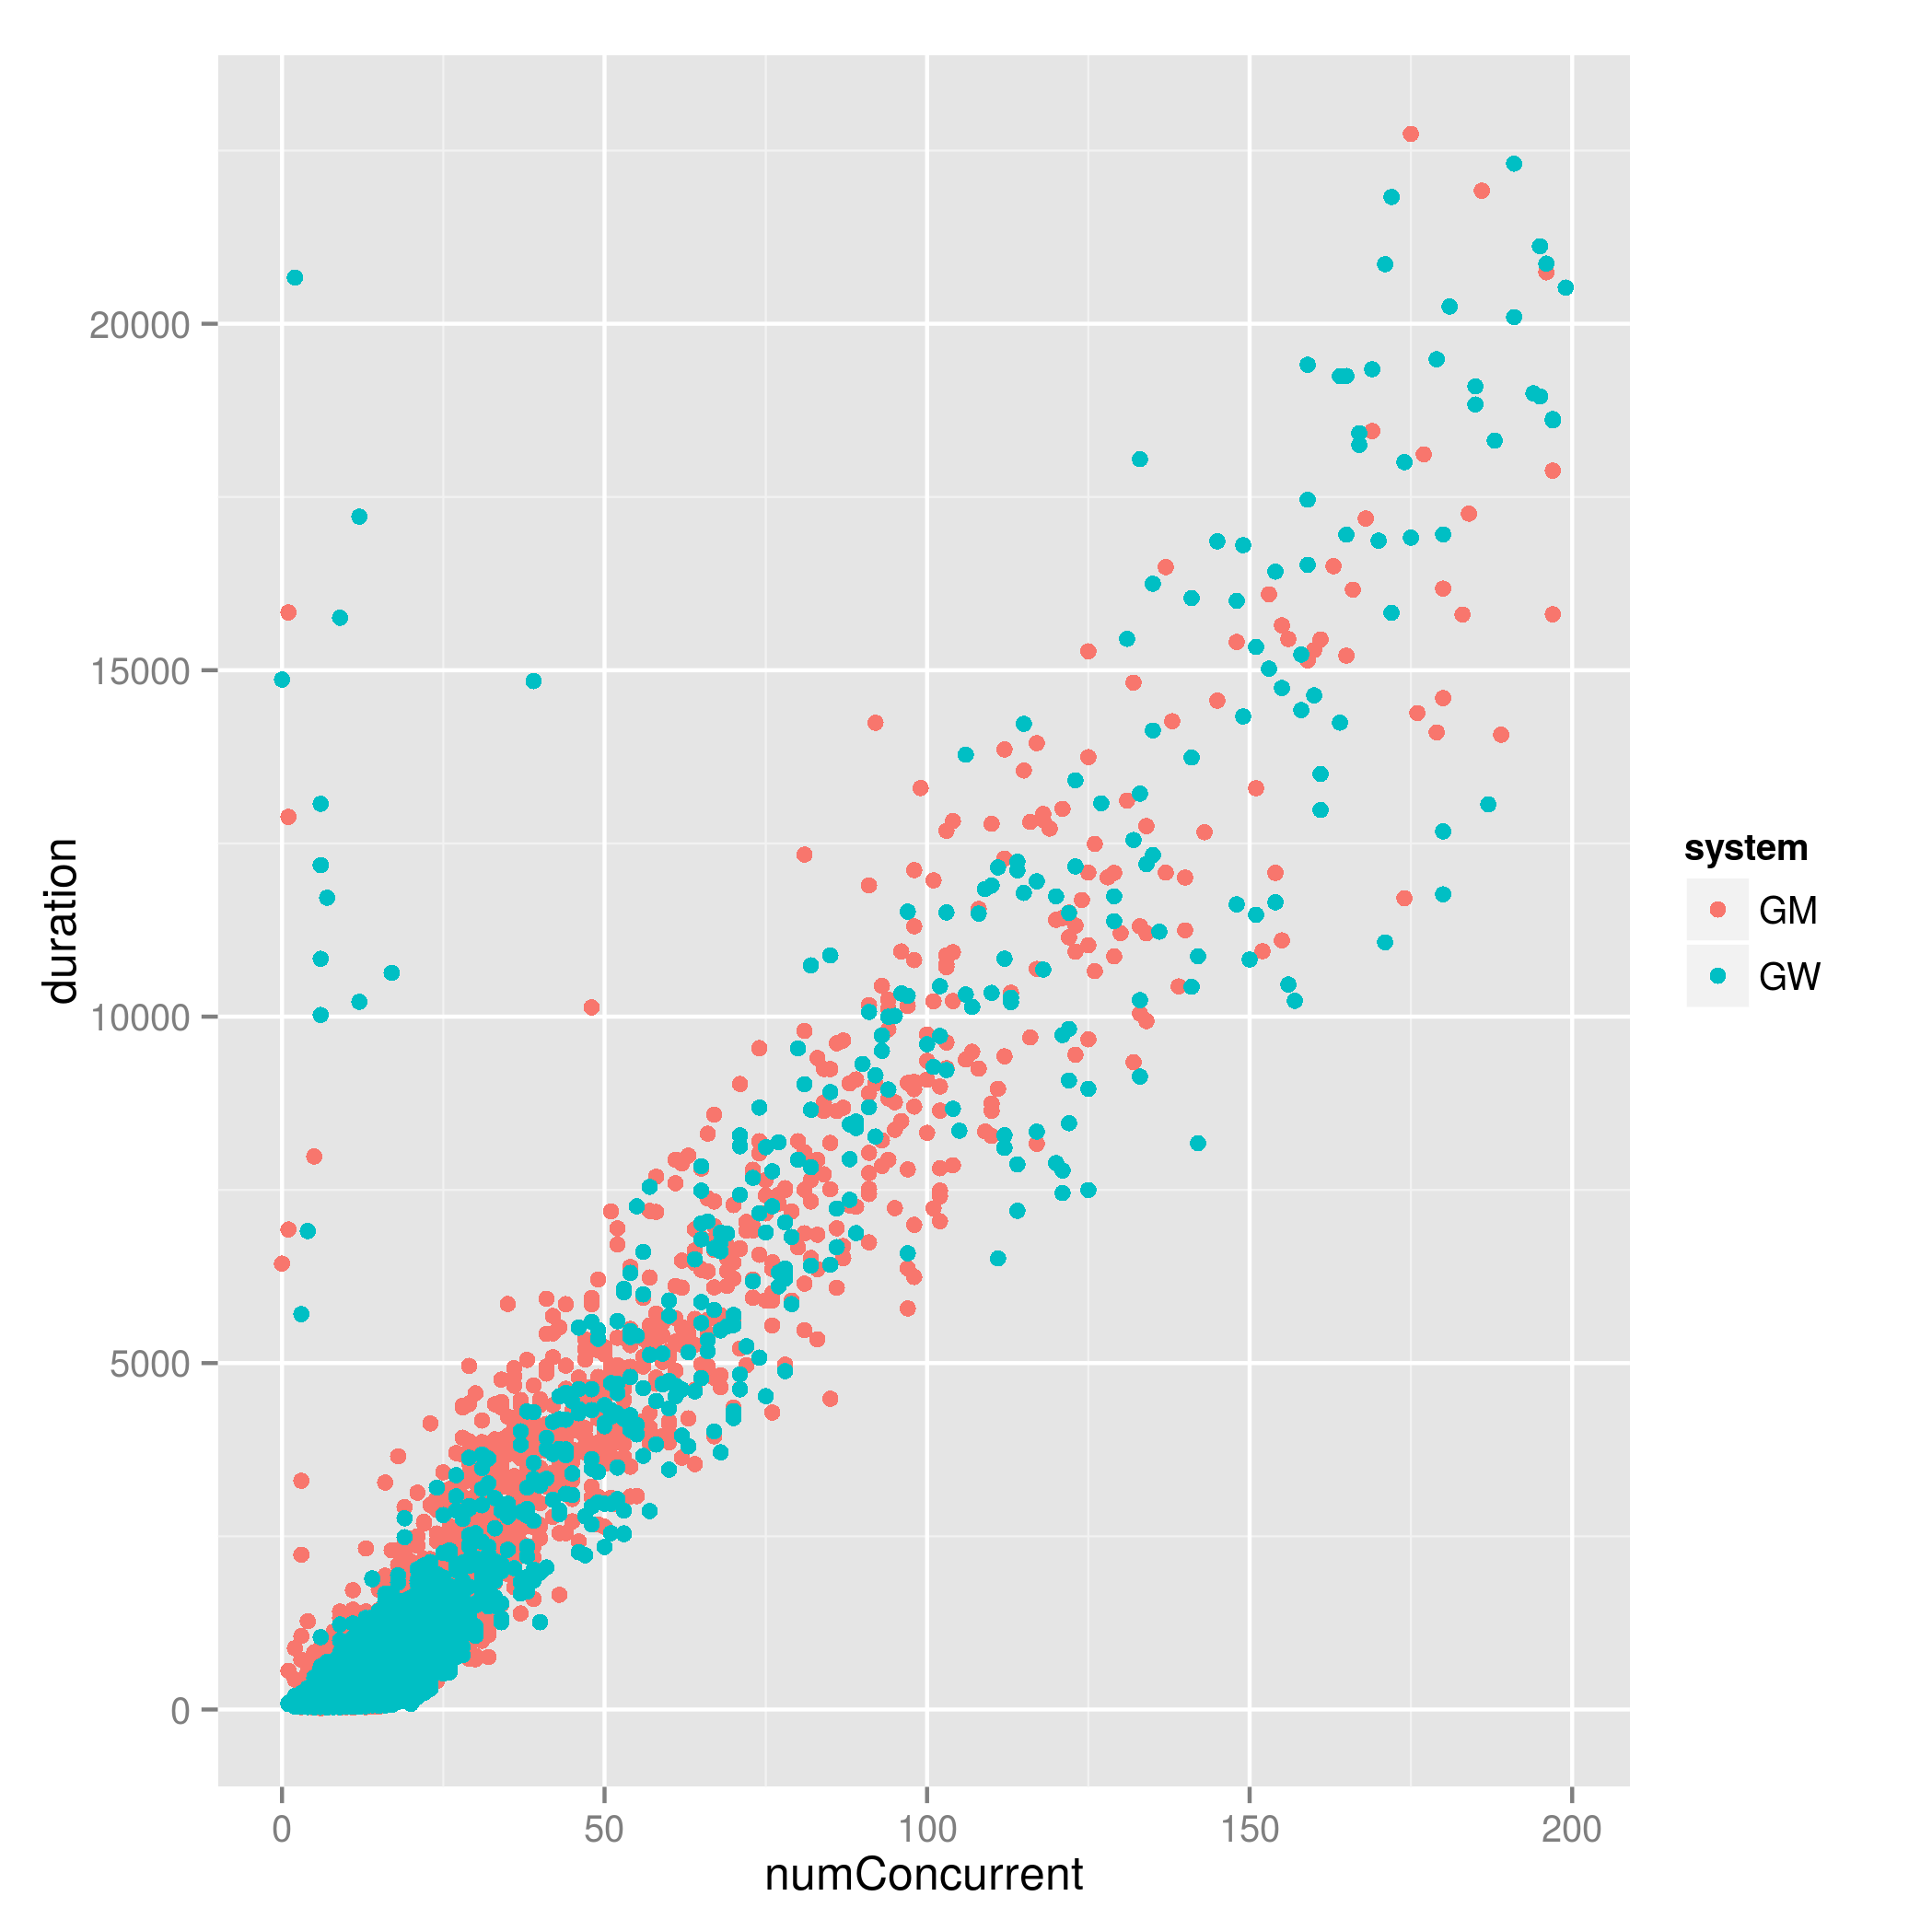
\includegraphics[width=0.60\textwidth]{images/mt3_g_numconcurrent.png}
  \caption{Results for the updated configuration.}
  \label{config4}
\end{figure}

While increased cache helped GeoWave performance some, brining average query duration down, it made massive improvement to GeoMesa performance and consistency.
The final difference in the query volume was only $30$\%.
Please see Figures \ref{config4}, \ref{config4distrogw}, and \ref{config4distrogm}.

\begin{figure}[h!tb]
  \centering
  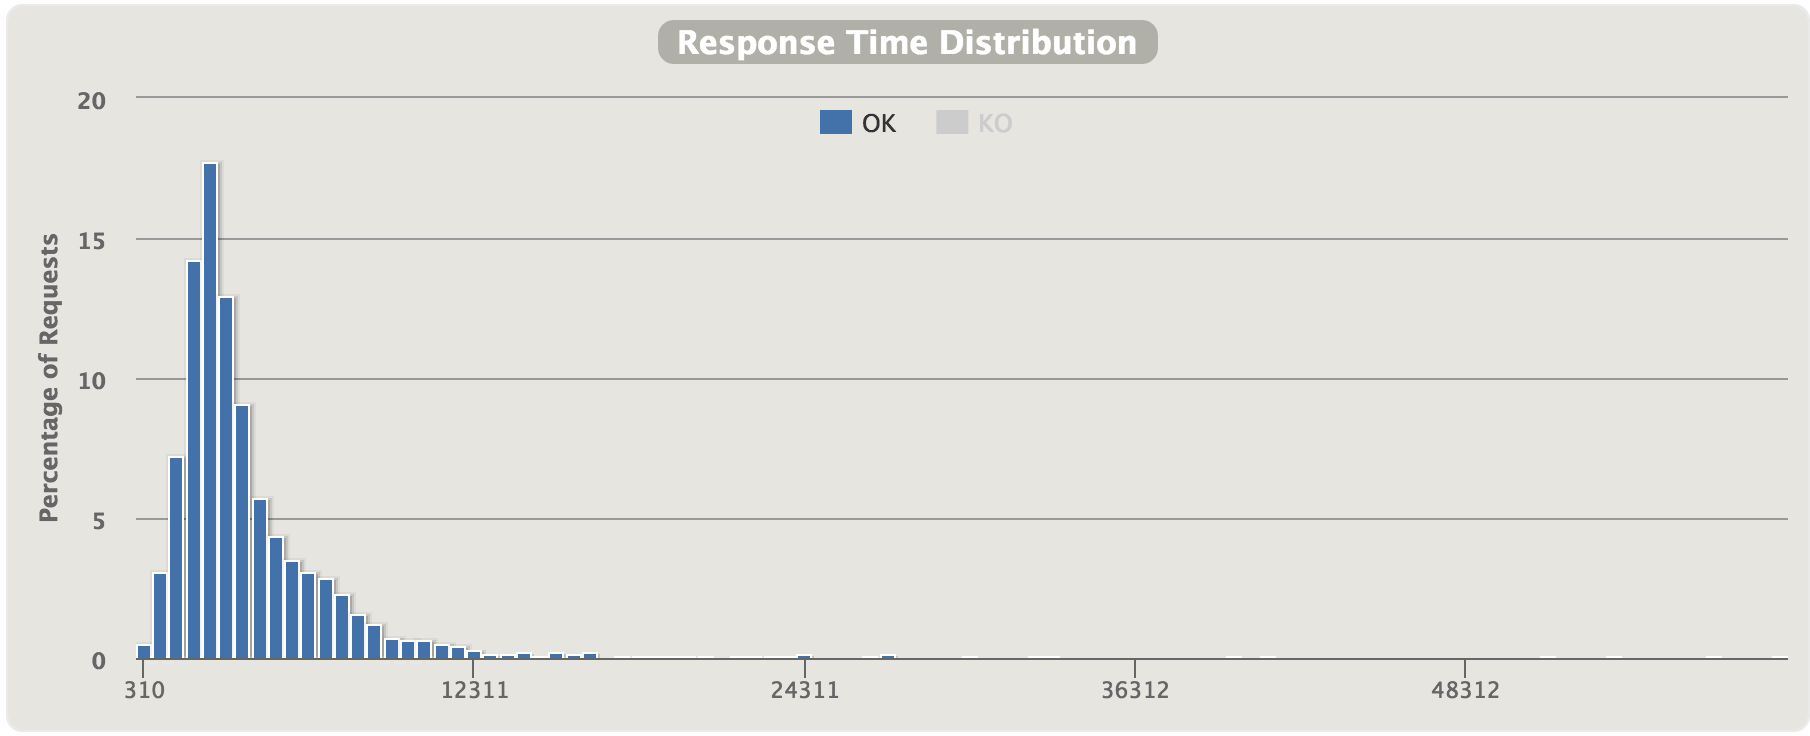
\includegraphics[width=0.60\textwidth]{images/mt4-gw.png}
  \caption{GeoWave/GDELT response times, configuration 3 with increased cache.}
  \label{config4distrogw}
\end{figure}

\begin{figure}[h!tb]
  \centering
  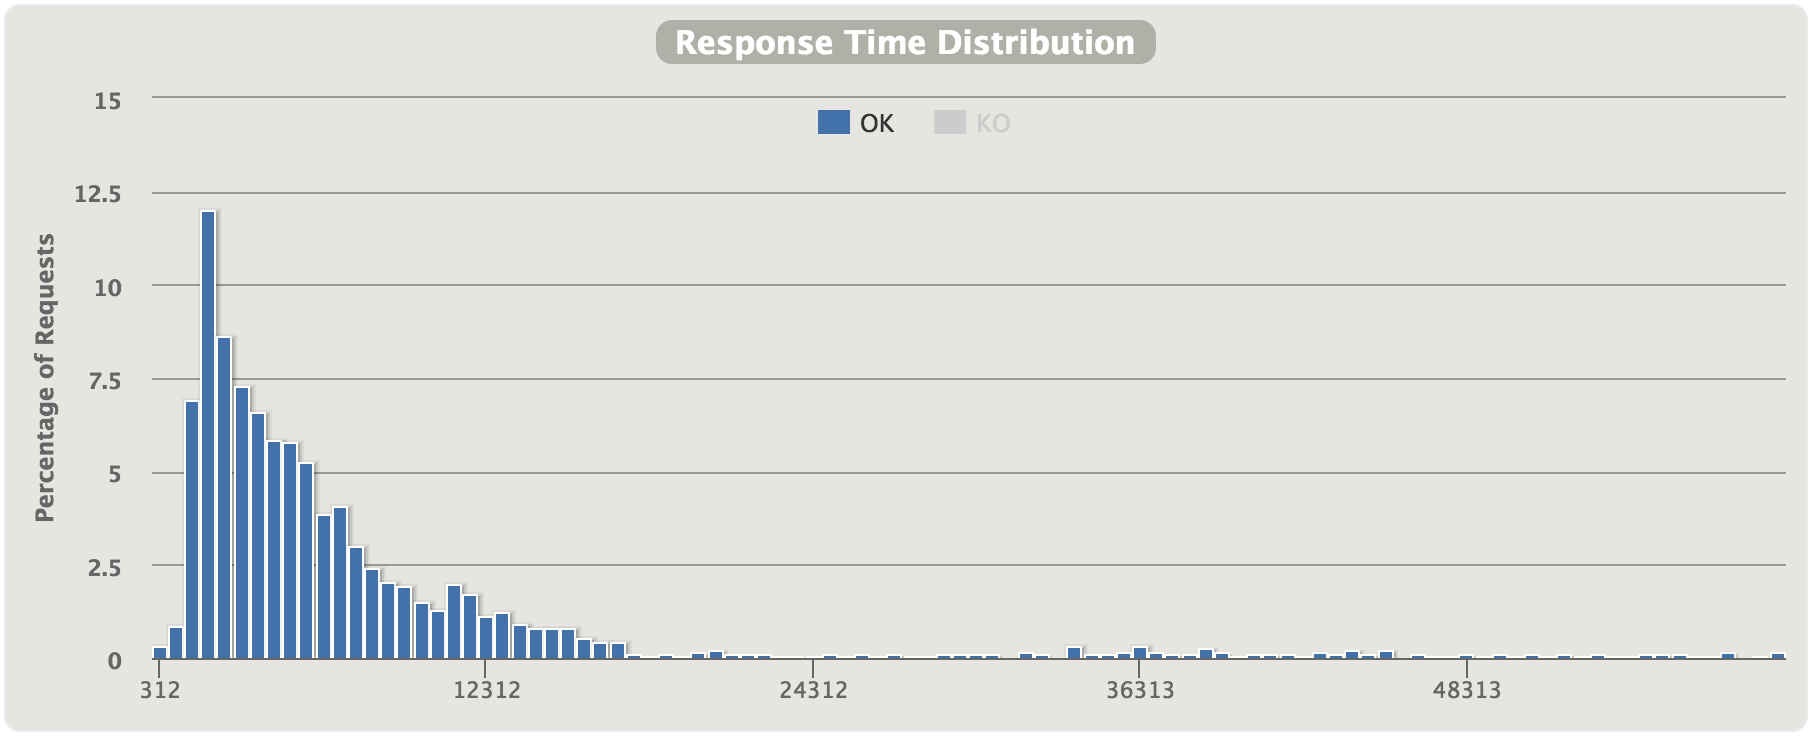
\includegraphics[width=0.60\textwidth]{images/gm-4.png}
  \caption{GeoMesa/GDELT response times, configuration 3 with increased cache.}
  \label{config4distrogm}
\end{figure}

It is difficult to attribute performance improvement in a distributed system but our speculation that remains consistent with our other findings is as follows: The failure cases seen in the initial set of results are likely due to garbage collection pressure as they were not reproduced with increased heap size.
Also it is clear that GeoMesa benefits significantly more from generous memory cache allocations than GeoWave.
In highly concurrent situations Accumulo performance is limited by tablet contention.
GeoWave more sophisticated query planner minimizes this contention by producing tighter query ranges.
Increasing the cache size also mitigates the tablet contention.

\subsection{Generated Tracks}

This dataset is densest around continental United States and covers a single year, with track length biased to be short.
We project a powers of $2$ pyramid over this area and query from pyramid level $4$ to $8$ with temporal selectivity ranging from $5$ days to $1$ month.
The generated query requests are biased towards lower levels of the pyramid, proportional to the number of grid cells at each level.
We test initially with $16$, $32$ concurrent connections.
Because we have seen from previous tests that six application servers is sufficient to handle query load from our cluster we only test against this configuration.

Generated tracks load tests allows us to test the performance of GeoMesa XZ3 versus GeoWave tiered Hilbert index.
Under heavy load with variance both over spatial and temporal selectivity both GeoMesa and GeoWave produced stable and reliable performance.
GeoWave delivers $60$\% higher request completion volume vs GeoMesa with $95$\textsuperscript{th} percentile response time being $7.5$ seconds.

\subsection{Test Results}

Increasing from $16$ to $32$ concurrent users produced nearly identical result counts per unit of time, $30$ minutes.
However, we see that it has increased latency for each request.

Most interesting are the response time distributions, which explain the difference in overall throughput.
GeoWave index trades minimum response time for more consistent and on average faster results.
Please see Figures \ref{geowave16}, \ref{geowave32}, \ref{geomesa16}, and \ref{geomesa32}.

\begin{figure}[h!tb]
  \centering
  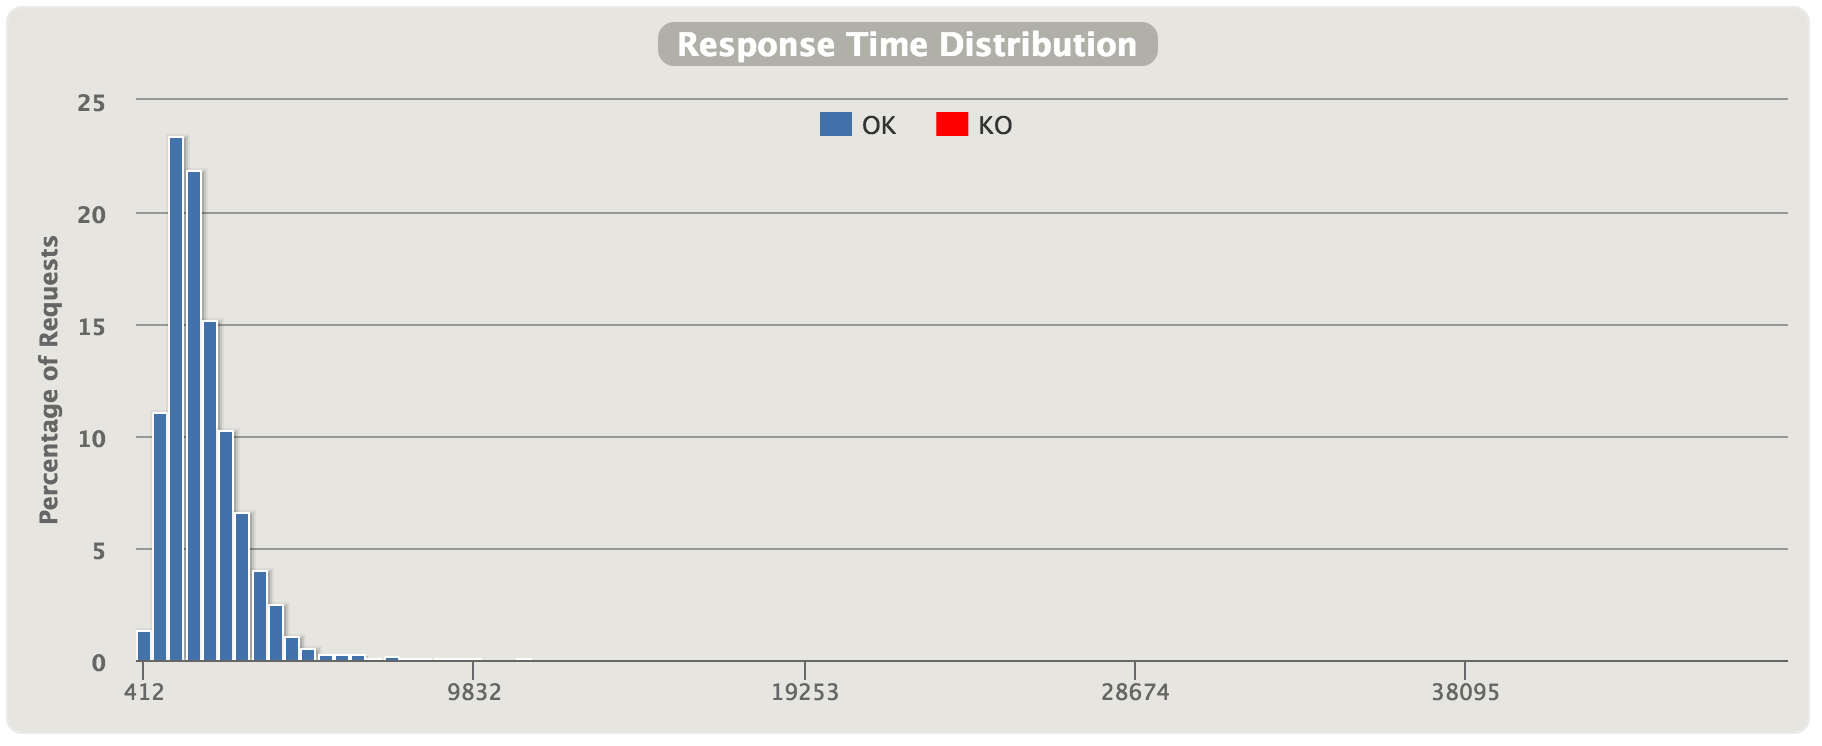
\includegraphics[width=0.60\textwidth]{../docs/img/multitenancy/gw-16-responses.png}
  \caption{GeoWave/Tracks response times, 16 users.}
  \label{geowave16}
\end{figure}

\begin{figure}[h!tb]
  \centering
  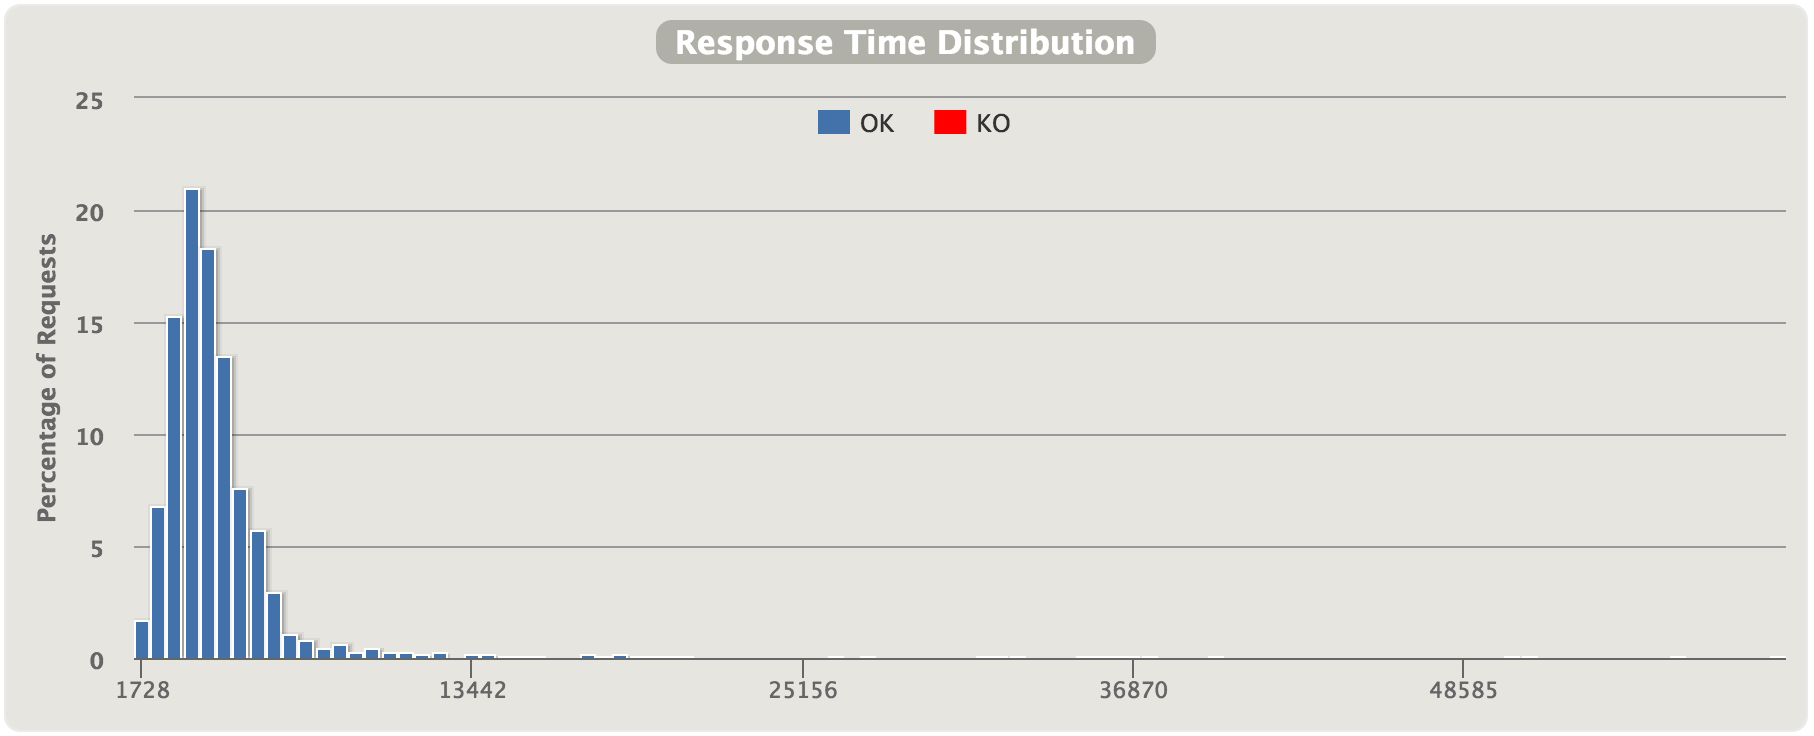
\includegraphics[width=0.60\textwidth]{../docs/img/multitenancy/gw-32-responses.png}
  \caption{GeoWave/Tracks response times, 32 users.}
  \label{geowave32}
\end{figure}

\begin{figure}[h!tb]
  \centering
  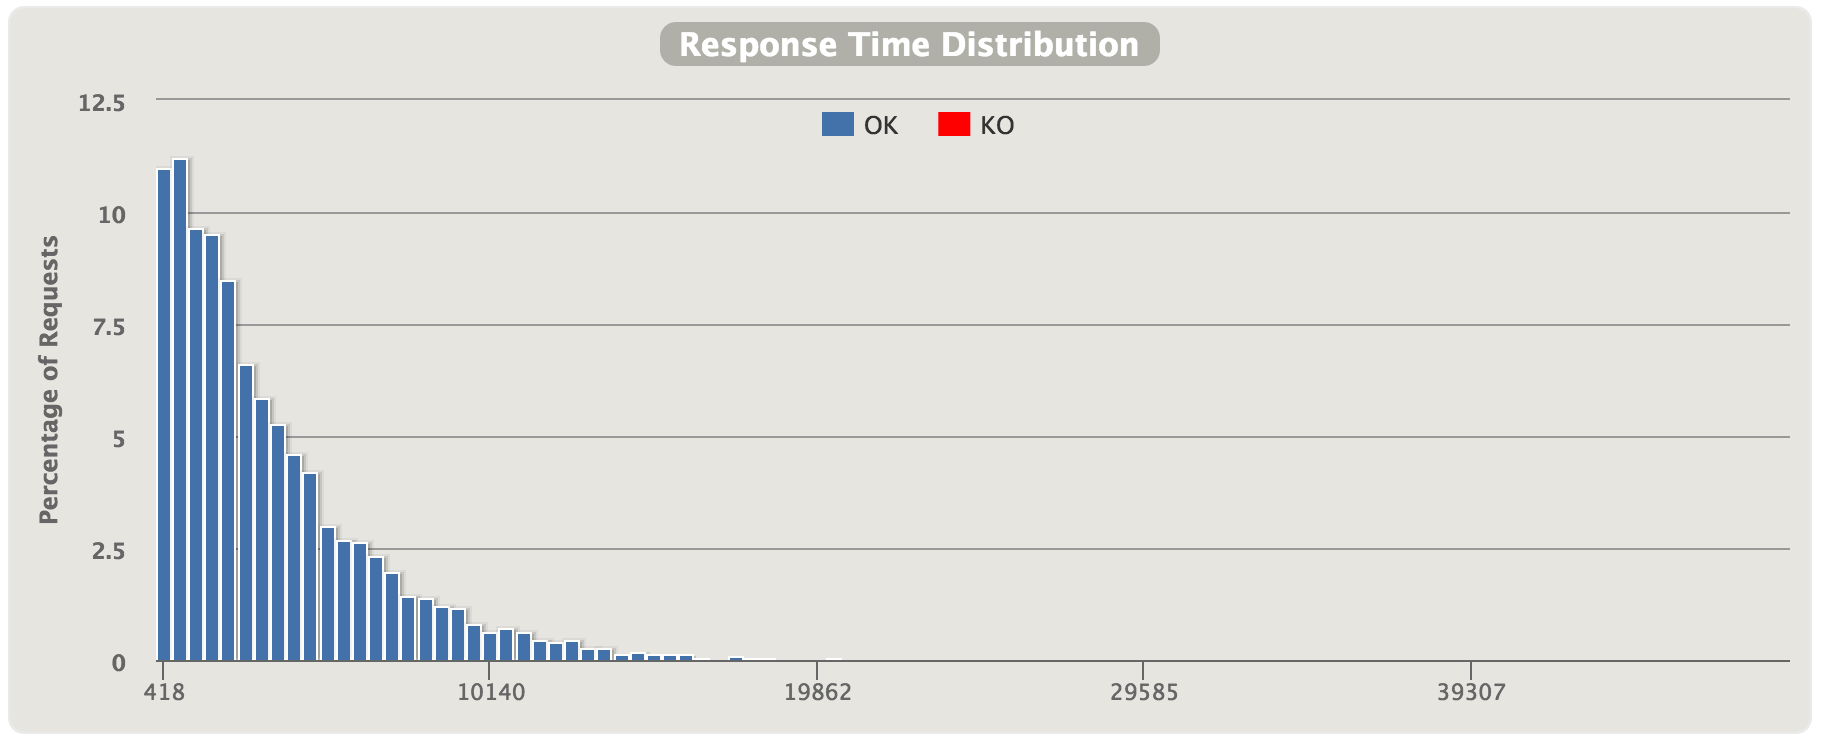
\includegraphics[width=0.60\textwidth]{../docs/img/multitenancy/gm-16-responses.png}
  \caption{GeoMesa/Tracks response times, 16 users.}
  \label{geomesa16}
\end{figure}

\begin{figure}[h!tb]
  \centering
  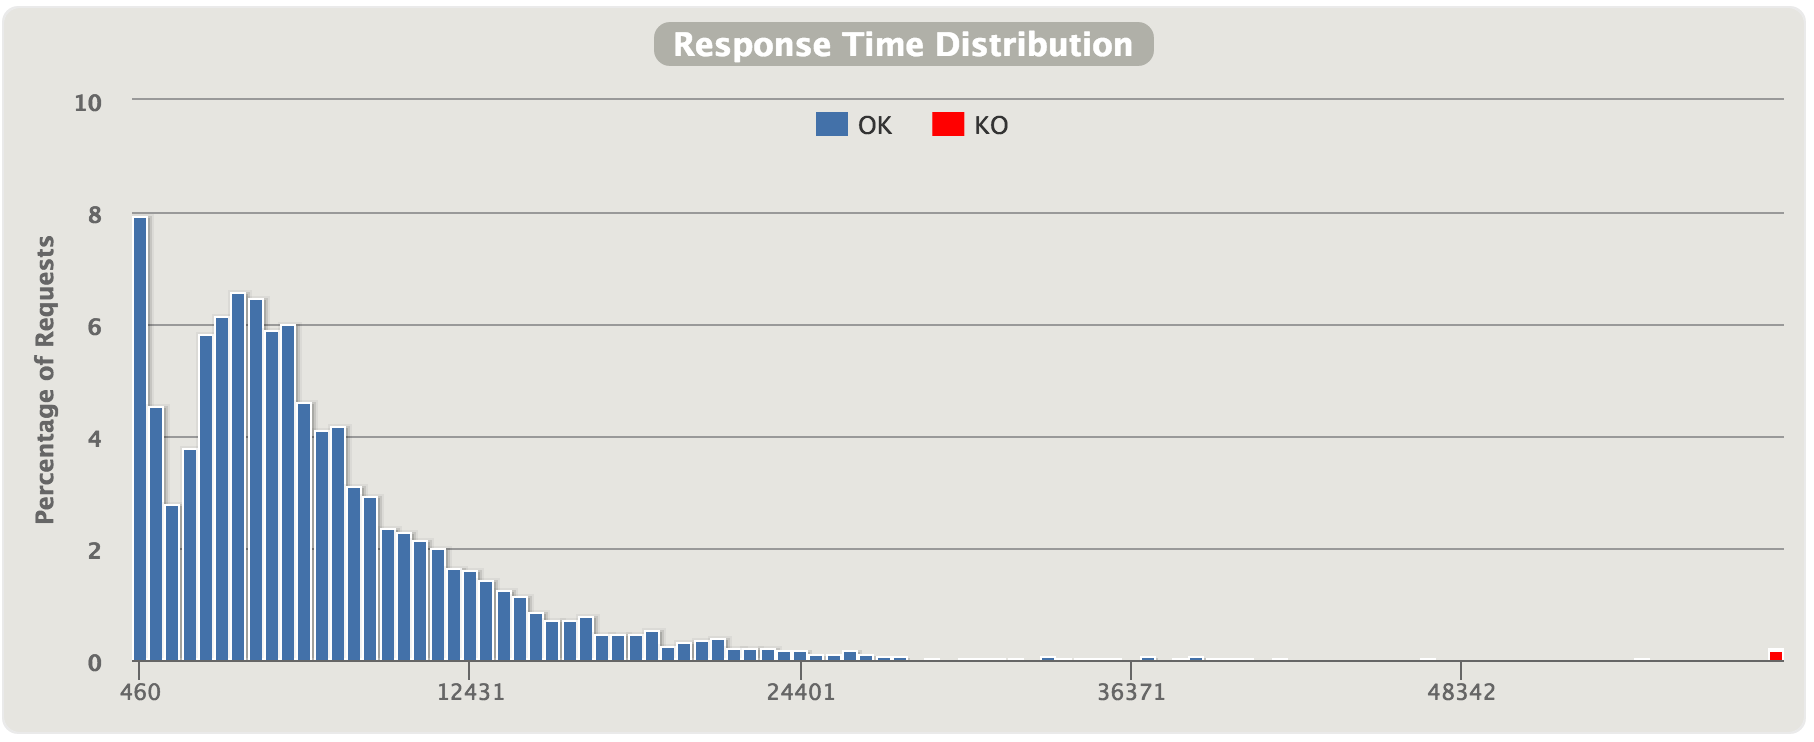
\includegraphics[width=0.60\textwidth]{../docs/img/multitenancy/gm-32-responses.png}
  \caption{GeoWave/Tracks response times, 32 users.}
  \label{geomesa32}
\end{figure}
